\chapter{Experiments} \label{experiments_chapter}

In previous chapters I have presented the dataset (chapter \ref{chapter:data}), and discussed challenges which arise from its properties (chapter \ref{chapPreproc}). Next I described the neural network architectures (chapter \ref{neural_nets_chapter}) which served as building blocks for the models introduced in chapter \ref{model_chapter}. Now I want to connect all the parts together, elaborate on the trainining of the models (e.g. used optimizer, calculated metrics, hyperparameter choice) and analyze their results.

Let me recap the main challenges we face, and hypothesize about the ideal generation system. Firstly, the target summaries are really long. The ideal system should remember what has already been generated and shouldn't produce duplications. Secondly, the targets contain a lot of facts based on the input structured data. The ideal system should copy these facts from the input and reduce \emph{hallucinations}. Lastly, the generated text should be as close to English as possible \emph{while meeting the requirements described previously}.

\section{Postprocessing}

The models are trained to generate lowercased Byte Pair Encoded sequences. During the postprocessing I merge the tokens belonging to one word together (e.g. \emph{"contribu$\star$ tor"} $\rightarrow$ \emph{"contributor"}), split the tokens of named entities (e.g. \emph{"LeBron\_James"} $\rightarrow$ \emph{"LeBron James"}) and uppercase the first letter of a sentence.

\section{Evaluation Methods}

During evaluation I want to measure which model resembles the hypothetical ideal model the most. To do so, I report the BLEU score \citep{papineni2002} of the postprocessed generated summaries on the validation and test sets. Although it is the gold standard, there are many people arguing against its usage as a performance metric \citep{celikyilmaz2021evaluation}, and I found that the networks producing more factually correct statements doesn't score better. Therefore I also manually evaluate a subset of the generated summaries.

\subsection{Manual Evaluation}

I used a pseudo random generator to pick 8 different data points, 4 from the validation and 4 from test set\footnote{Specifically samples $132$, $319$, $475$ and $709$ from the validation set and samples $16$, $247$, $585$ and $671$ from the test set}. I looked at the factual correctness (how many of the generated numbers describing team and player statistics are based on the input tabular data), and factual recall (how many of the entities mentioned in the gold summaries are present in the generated ones). Due to time-requirements of the process, only the best model\footnote{In the respective sections I explain why I think the selected model is the best one.} is manually evaluated. Therefore manual evaluation should show the differences between approaches and architectures rather than between variations of the same model.

\subsection{Ommited Evaluation Methods}

\citep{wiseman2017} proposed three custom automated metrics to evaluate the performance of their models. They call them \emph{Content Selection} ("how well the generated document matches the gold document in terms of selecting which records to generate"), \emph{Relation Generation} ("how well the system is able to generate text containing factual (i.e., correct) records") and \emph{Content Ordering} ("how well the system orders the records it chooses to discuss"). The metrics are implemented in outdated neural network framework \emph{Torch} and I wasn't able to execute it on my computers. After discussions with my advisor we agreed to not adopt these methods.

\section{Baseline Model}

At first I would like to summarize my expectations. \citep{wiseman2017} note that even models with explicit copy mechanisms tend to \emph{hallucinate} the facts. However they do not show the results of any baseline without copying. We expect the baseline to generate a fairly good English, even though the summaries should not be factually correct.

I searched through the hyperparameter space (possible combinations of learning rates, dropout probability $p$, hidden state dimensionality etc.) until the generated language as well as the numerical results haven't fulfilled the expectations at least by half.

The overall architecture of the baseline model is discussed in section \ref{section:baseline_model}. Figure \ref{figure:hyperparameters_baseline} shows the hyperparameter choice for discussed baseline models.

\begin{figure}[h]
    \scalebox{0.8}{
    \begin{tikzpicture}
    \node(embeddings) [] {
        \small
        \begin{tabular}{ll}
            \toprule
            {} & \textbf{Embedding} \\
            \pulrad{\textbf{Token}} & \textbf{Dimensionality} \\
            \midrule
            \textbf{$record.type$} & 300 \\
            \textbf{$record.home\_away$} & 300 \\
            \textbf{$record.value$} & 600 \\
            \textbf{$record.entity$} & 600 \\
            \textbf{$summary\ token$} & 600
        \end{tabular}
    };
    \node(hidden) [above left=-20.7mm and 5mm of embeddings] {
        \small
        \begin{tabular}{ccc}
            \toprule
            \textbf{Hidden States} & {} & {} \\
            \textbf{Dimensionality} & \pulrad{\textbf{Learning Rate}} & \pulrad{\textbf{Batch Size}} \\
            \midrule
            600 & 0.001 & 16
        \end{tabular}
    };
    \end{tikzpicture}
    }
    \caption{Hyperparameter settings for baseline models.} \label{figure:hyperparameters_baseline}
\end{figure}

The first baseline model is trained without any regularization, the second one with dropout on the output LSTM units with $p_{dropout} = 0.3$ (the probability that the unit is dropped is $0.3$) and scheduled sampling with constant rate of $0.8$ (the probability that the gold output from the previous timestep is used as the actual input is $0.8$).

\subsection{Results}

Baseline model wasn't able to capture the relationships between the input tabular data and the output summaries (the best configuration achieved perplexity $10.59$). We found that dropout helps to reduce overfitting while scheduled sampling improved the quality of the generated summaries. (We present only models which achieved reasonable performance.) The quality of generated summaries is further improved with beam search. Although the statement contradicts the calculated BLEU scores (as the score decreased after introducing beam search), the summaries contain more natural language and less repetitions. The expectations are fulfilled in terms of \emph{hallucinations}, as the model makes up \emph{almost all the factual statements}.

\begin{table}[h]
    \centering
    \scalebox{0.8}{
    \begin{tabular}{lccccc}
        \toprule
        {} & \textbf{Validation} & \textbf{Validation} & \textbf{Test} & \textbf{Entity} & \textbf{Correct} \\
        \pulrad{\textbf{Model}} & \textbf{Perplexity} & \textbf{BLEU} & \textbf{BLEU} & \textbf{Recall} & \textbf{Facts} \\
        \midrule
        BN$_G$ & {} & 9.04 & 9.10 & -- & -- \\
        BN$_{B5}$ & \pulrad{12.68} & 8.73 & 8.55 & -- & -- \\
        \hline
        BR$_G$ & {} & 10.0 & 10.47 & -- & -- \\
        BR$_{B5}$ & \pulrad{10.59} & 9.99 & 10.6 & 37.35\% & 8.03\% \\
        \bottomrule
        \multicolumn{4}{l}{\footnotesize{$_{G}$ - Greedy Decoding}} \\
        \multicolumn{4}{l}{\footnotesize{$_{B5}$ - Beam search decoding, beam size $=5$}} \\
        \multicolumn{4}{l}{\footnotesize{BN - Baseline, non-regularized}} \\
        \multicolumn{4}{l}{\footnotesize{BR - Baseline, regularized (dropout $0.3$, scheduled sampling $0.8$)}}
    \end{tabular}
    }
    \caption{Performance metrics on the baseline models.} \label{table:metrics_baseline}
\end{table}

Figure \ref{figure:baseline_generated} shows an example generated by the regularized baseline model with beam search decoding. We observe\footnote{We opted to not show the same tabular information multiple times. A part of the table corresponding to the generated summary can be found in figure \ref{figure:samplesummary}} that the score, the winning-loosing records\footnote{\emph{"The Raptors ( 21 - 15)"} means that Raptors have won $21$ matches and lost $15$ matches this season.} as well as all the individual statistics are \emph{hallucinated}. We found that the model repeatedly (over multiple observed summaries) mentions the same players and uses the same numbers. This experiment thus supports our assumptions. Statistics in table \ref{table:metrics_baseline} show that only about $8$ \% of the numbers aren't \emph{hallucinated} and that the recall is lower than $35$ \%. Therefore we can conclude that model learned to produce probable numbers and names of star players of the respective teams. 


\begin{figure}[h]
    \scalebox{0.85}{
    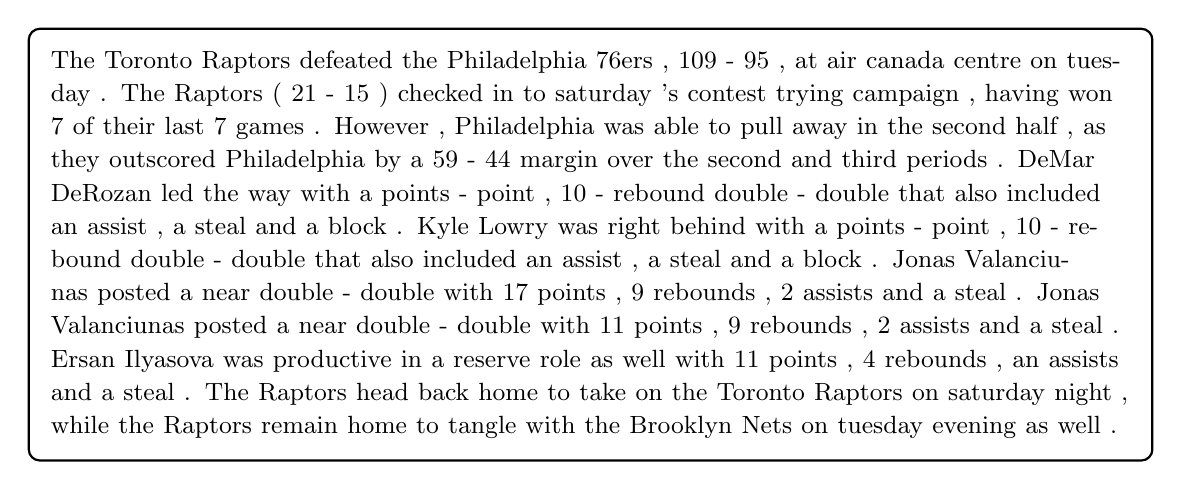
\begin{tikzpicture}
    \node(summary) [rectangle, draw,thick,fill=blue!0,text width=39em, rounded corners, inner sep =8pt, minimum height=1em]{
        \baselineskip=100pt
        \small
        The Toronto Raptors defeated the Philadelphia 76ers , 109 - 95 , at air canada centre on tuesday . The Raptors ( 21 - 15 ) checked in to saturday 's contest trying campaign , having won 7 of their last 7 games . However , Philadelphia was able to pull away in the second half , as they outscored Philadelphia by a 59 - 44 margin over the second and third periods . DeMar DeRozan led the way with a points - point , 10 - rebound double - double that also included an assist , a steal and a block . Kyle Lowry was right behind with a points - point , 10 - rebound double - double that also included an assist , a steal and a block . Jonas Valanciunas posted a near double - double with 17 points , 9 rebounds , 2 assists and a steal . Jonas Valanciunas posted a near double - double with 11 points , 9 rebounds , 2 assists and a steal . Ersan Ilyasova was productive in a reserve role as well with 11 points , 4 rebounds , an assists and a steal . The Raptors head back home to take on the Toronto Raptors on saturday night , while the Raptors remain home to tangle with the Brooklyn Nets on tuesday evening as well .
    };
    \end{tikzpicture} }
    \caption{\centering A summary generated by the baseline model. The corresponding gold summary and input table is shown in figure \ref{figure:samplesummary}.} \label{figure:baseline_generated}
\end{figure}

\section{Joint-Copy Model}

The Joint-Copy Model is expected to produce more factually correct statements. \citep{wiseman2017} select this model as their baseline. Due to massive preprocessing that we introduced, the results we obtained aren't comparable to theirs. (E.g. Wiseman et al. report BLEU $10.41$ while we obtained similar scores with \emph{simpler baseline model}.)

The additional complexity of the model increases the memory demands. The\-refore we use lower dimensional embeddings, hidden states and smaller batch size as presented in figure \ref{figure:hyperparameters_copy_low_lr} to be able to train on the GPUs on the AIC. Compared to the baseline model we obtained the best results when training with $5$-times lower learning rate. Regularization methods didn't provide any significant advantage over the unregularized case.

\begin{figure}[h]
    \scalebox{0.8}{
    \begin{tikzpicture}
    \node(embeddings) [] {
        \small
        \begin{tabular}{ll}
            \toprule
            {} & \textbf{Embedding} \\
            \pulrad{\textbf{Token}} & \textbf{Dimensionality} \\
            \midrule
            \textbf{$record.type$} & 300 \\
            \textbf{$record.home\_away$} & 300 \\
            \textbf{$record.value$} & 500 \\
            \textbf{$record.entity$} & 500 \\
            \textbf{$summary\ token$} & 500
        \end{tabular}
    };
    \node(hidden) [above left=-20.7mm and 5mm of embeddings] {
        \small
        \begin{tabular}{ccc}
            \toprule
            \textbf{Hidden States} & {} & {} \\
            \textbf{Dimensionality} & \pulrad{\textbf{Learning Rate}} & \pulrad{\textbf{Batch Size}} \\
            \midrule
            500 & 0.0002 & 8
        \end{tabular}
    };
    \end{tikzpicture}
    }
    \caption{Hyperparameter settings for joint-copy models.} \label{figure:hyperparameters_copy_low_lr}
\end{figure}

\subsection{Results}

We see the first major improvement in the BLEU score (more than 2 points) as well as in the manually evaluated metrics (almost $6$-times better factual correctness). However the model fails in recognition of the structure of the table.

While it is able to copy facts, many times it copies statistics of wrong players (e.g. it learns that most of the time $5$-th player from the input records is most important, therefore it mentions the $5$-th player even if he scored unremarkable amount of points).

We also spotted that model learned that it is more probable that home team wins. Therefore it produces sentence similar to \emph{"The Denver Nuggets ( 11 - 17 ) defeated the Los Angeles Lakers ( 5 - 23 ) 111 - 107 on friday at the pepsi center in Denver . "} even if the score was reversed (\emph{107 - 111} in favour of the Lakers).

Also the model relatively often generates a sequence of tokens which cannot be seen in the training data which causes \emph{cycling} (model generates one sentence multiple times), which results in exceeding the maximal allowed length of a summary (We don't allow the model to generate longer sequence than the longest one seen in the dataset (849 tokens)). The phenomenon can be seen in figure \ref{figure:copy_low_lr_generated}.

Contrary to observations on the baseline model neither greedy decoding nor beam search managed to significantly outperform the other method.

\begin{table}[h]
    \centering
    \scalebox{0.8}{
    \begin{tabular}{lccccc}
        \toprule
        {} & \textbf{Validation} & \textbf{Validation} & \textbf{Test} & \textbf{Entity} & \textbf{Correct} \\
        \pulrad{\textbf{Model}} & \textbf{Perplexity} & \textbf{BLEU} & \textbf{BLEU} & \textbf{Recall} & \textbf{Facts} \\
        \midrule
        Copy$_G$ & {} & 12.48 & 12.6 & 37.35\% & 47.29\% \\
        Copy$_{B5}$ & \pulrad{9.87} & 12.19 & 12.5 & 39.76\% & 47.13\% \\
        \bottomrule
        \multicolumn{6}{l}{\footnotesize{Copy - Joint-Copy model}} \\
        \multicolumn{4}{l}{\footnotesize{$_{G}$ - Greedy Decoding}} \\
        \multicolumn{4}{l}{\footnotesize{$_{B5}$ - Beam search decoding, beam size $=5$}} \\
    \end{tabular}
    }
    \caption{Performance metrics on the joint-copy models.} \label{table:metrics_copy_low_lr}
\end{table}

\begin{figure}[h]
    \scalebox{0.85}{
    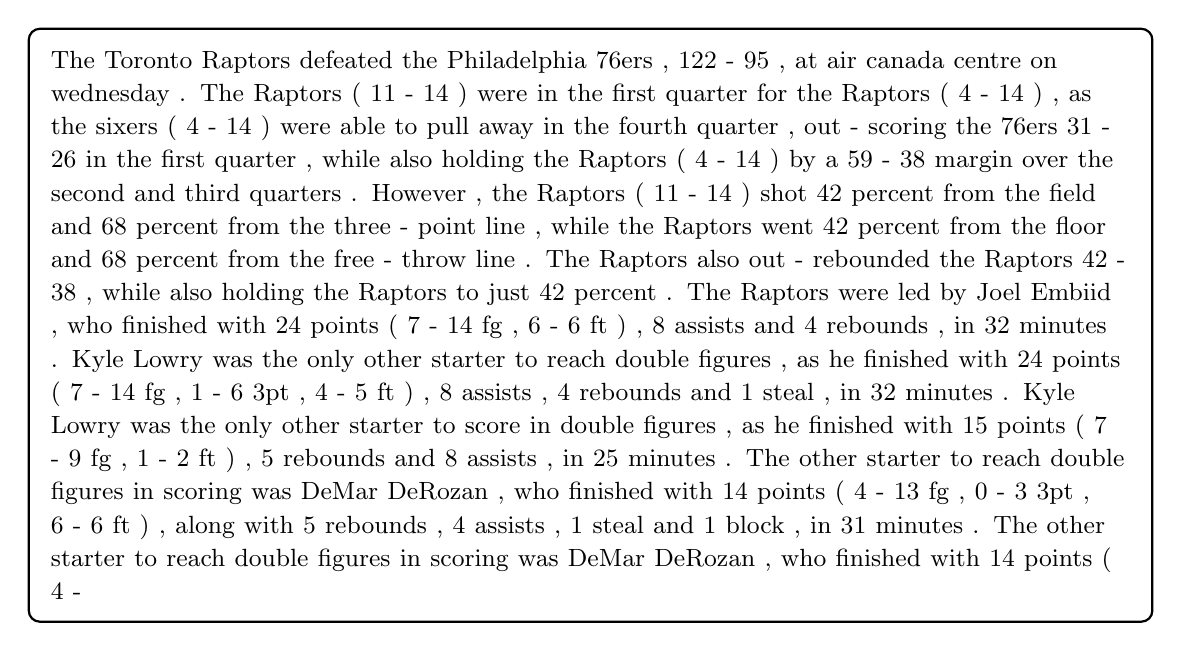
\begin{tikzpicture}
    \node(summary) [rectangle, draw,thick,fill=blue!0,text width=39em, rounded corners, inner sep =8pt, minimum height=1em]{
        \baselineskip=100pt
        \small
        The Toronto Raptors defeated the Philadelphia 76ers , 122 - 95 , at air canada centre on wednesday . The Raptors ( 11 - 14 ) were in the first quarter for the Raptors ( 4 - 14 ) , as the sixers ( 4 - 14 ) were able to pull away in the fourth quarter , out - scoring the 76ers 31 - 26 in the first quarter , while also holding the Raptors ( 4 - 14 ) by a 59 - 38 margin over the second and third quarters . However , the Raptors ( 11 - 14 ) shot 42 percent from the field and 68 percent from the three - point line , while the Raptors went 42 percent from the floor and 68 percent from the free - throw line . The Raptors also out - rebounded the Raptors 42 - 38 , while also holding the Raptors to just 42 percent . The Raptors were led by Joel Embiid , who finished with 24 points ( 7 - 14 fg , 6 - 6 ft ) , 8 assists and 4 rebounds , in 32 minutes . Kyle Lowry was the only other starter to reach double figures , as he finished with 24 points ( 7 - 14 fg , 1 - 6 3pt , 4 - 5 ft ) , 8 assists , 4 rebounds and 1 steal , in 32 minutes . Kyle Lowry was the only other starter to score in double figures , as he finished with 15 points ( 7 - 9 fg , 1 - 2 ft ) , 5 rebounds and 8 assists , in 25 minutes . The other starter to reach double figures in scoring was DeMar DeRozan , who finished with 14 points ( 4 - 13 fg , 0 - 3 3pt , 6 - 6 ft ) , along with 5 rebounds , 4 assists , 1 steal and 1 block , in 31 minutes . The other starter to reach double figures in scoring was DeMar DeRozan , who finished with 14 points ( 4 -
    };
    \end{tikzpicture} }
    \caption{\centering A summary generated by the joint-copy model. The corresponding gold summary and input table is shown in figure \ref{figure:samplesummary}.} \label{figure:copy_low_lr_generated}
\end{figure}

\section{Content Selection Encoder with Joint-Copy Decoder}

\citep{puduppully2019datatotext} introduced two new concepts. The first one, the Content Selection (CS) (discussed in section \ref{subsection:content_selection}) uses self-attention to incorporate \emph{context awareness}. Basically it should mean that the encoded record representation should be aware about the most important records related to itself. \citep{puduppully2019datatotext} report that CS alone contributes to the quality of the generated summaries. We expect the model with CS to resolve the problem of mixing statistical information of multiple players.

The hyperparameter configuration rests the same as in Joint-Copy model (figure \ref{figure:hyperparameters_copy_low_lr}).

\subsection{Results}

The summaries produced by the model are richer in structure, as they mention more entities from the input tables ($44.58$ \% vs $39.76$ \% for the Copy model). However we observe that many times model doesn't copy the players name (it only learns to copy numbers). E.g. it generates a sentence \emph{"The Raptors were led by DeMar DeRozan , who finished with a team - high of 26 points ( 9 - 16 fg , 0 - 2 3pt , 8 - 9 ft ) , to go along with 7 rebounds and 5 assists ."} where there would be $8 / 9$ numbers correct if the name wasn't \emph{DeMar DeRozan} but \emph{Marc Gasol}. This causes the model to score less on the factual correctness metric ($42.22$ \% vs $47.13$ \% for the Copy Model). Regarding BLEU score we see an improvement of about $1$ point.

\begin{table}[h]
    \centering
    \scalebox{0.8}{
    \begin{tabular}{lccccc}
        \toprule
        {} & \textbf{Validation} & \textbf{Validation} & \textbf{Test} & \textbf{Entity} & \textbf{Correct} \\
        \pulrad{\textbf{Model}} & \textbf{Perplexity} & \textbf{BLEU} & \textbf{BLEU} & \textbf{Recall} & \textbf{Facts} \\
        \midrule
        CopyCS$_G$ & {} & 13.53 & 13.62 & -- & -- \\
        CopyCS$_{B5}$ & \pulrad{9.93} & 13.54 & 13.96 & 44.58\% & 42.22\% \\
        \bottomrule
        \multicolumn{4}{l}{\footnotesize{CopyCS - Joint-Copy decoder $+$ Content Selection encoder}} \\
        \multicolumn{4}{l}{\footnotesize{$_{G}$ - Greedy Decoding}} \\
        \multicolumn{4}{l}{\footnotesize{$_{B5}$ - Beam search decoding, beam size $=5$}} \\
    \end{tabular}
    }
    \caption{Performance metrics on the joint-copy model with content selection encoder.} \label{table:metrics_copy_content_selection}
\end{table}

I would like to note that I don't think I came even close to the apex of the performance of this configuration as many summaries still show indications of underfitting (e.g. sequences like \emph{"TEAM-A defeated TEAM-A"}). Therefore I do not show an example of the summary generated by the model (as it contains sentences of the same quality as the ones generated by the joint-copy model).

\section{Content Selection and Planning}

The second concept introduced by \citep{puduppully2019datatotext} is the Content Planning Decoder (discussed in section \ref{subsection:content_planning}). The generation is divided into two parts. In the first one, we generate a sequence of pointers to the input records which contain the most essential information from the table. In the second phase we generate the summary according to records pointed to by the extracted pointers. Multitude of added architectures (content selection attention, content planning attention, content planning LSTM) increased even more the memory demands. Therefore we again reduced the embedding and hidden state dimensionalities (figure \ref{figure:hyperparameters_content_selection_and_planning}).

\begin{figure}[h]
    \scalebox{0.8}{
    \begin{tikzpicture}
    \node(embeddings) [] {
        \small
        \begin{tabular}{ll}
            \toprule
            {} & \textbf{Embedding} \\
            \pulrad{\textbf{Token}} & \textbf{Dimensionality} \\
            \midrule
            \textbf{$record.type$} & 300 \\
            \textbf{$record.home\_away$} & 300 \\
            \textbf{$record.value$} & 450 \\
            \textbf{$record.entity$} & 450 \\
            \textbf{$summary\ token$} & 450
        \end{tabular}
    };
    \node(hidden) [above left=-20.7mm and 5mm of embeddings] {
        \small
        \begin{tabular}{ccc}
            \toprule
            \textbf{Hidden States} & {} & {} \\
            \textbf{Dimensionality} & \pulrad{\textbf{Learning Rate}} & \pulrad{\textbf{Batch Size}} \\
            \midrule
            450 & 0.0002 & 8
        \end{tabular}
    };
    \end{tikzpicture}
    }
    \caption{Hyperparameter settings for content selection and planning models.} \label{figure:hyperparameters_content_selection_and_planning}
\end{figure}

Content Planning reduces the size of the table, and \emph{arranges} the records into the same order in which they appear in the gold summary. There are two aspects of this solution which should help the model to generate better summaries. Firstly, the input sequences of records become less complex (the maximal length of content plan is $92$ compared to more than $800$ for the original tables). Secondly, the records are ordered in the same way as they should appear in the summary. \citep{puduppully2019datatotext} show that this approach led them to really promising results (e.g. they obtained BLEU score of about $16$).

\subsection{Results}

During generation we applied two different settings. Firstly we ignore the outputs from the Content Planning Decoder and use the \emph{gold content plan}. (Since we have the gold content plans only for the training and validation parts of the dataset, the reported metrics are calculated only on the validation part) We can see that with gold content plans model mentions more than $70$\% of the entities that also appear in the gold summaries (we believe that the number would increase with better quality of the gold content plans\footnote{\citep{puduppully2019datatotext} extract the content plans with specialized information extraction system, and they claim that "strictly speaking, we cannot talk about gold content plans".}).

Figure \ref{figure:gold_cp_generated} is a good example of the summaries which are generated from the \emph{gold content plans}. Gold summary mentions 13 entities, out of which 12 are mentionned in the generated one. The generated text contains 39 numerical values out of which 31 are correct. The model learned to place the information about the entites in right\footnote{The same order as in the gold summaries.} order, and to copy numbers related to entites. Although still many flaws persist. I.e. the model generated 3 times the same information about \emph{Richaun Holmes}\footnote{Let me note that there is a numerical value \emph{"$11$ points"} which is counted 3 times. (Therefore $3$ is added to both \emph{all the numerical values} and \emph{correct numerical values}. This causes wrong reduplicated information to decrease the manual metrics more.)} Another problem demonstrated in the summary is that model mixed up records about Toronto and about Philadelphia (e.g. model generates sentence : \emph{"Defense was key for Toronto , as they held Philadelphia to 55 percent from the field and 68 percent from three - point range ."}, however 55\% shooting for 2pt and 68\% shooting for 3pt are the statistics related to Toronto).

\begin{figure}[h]
    \scalebox{0.85}{
    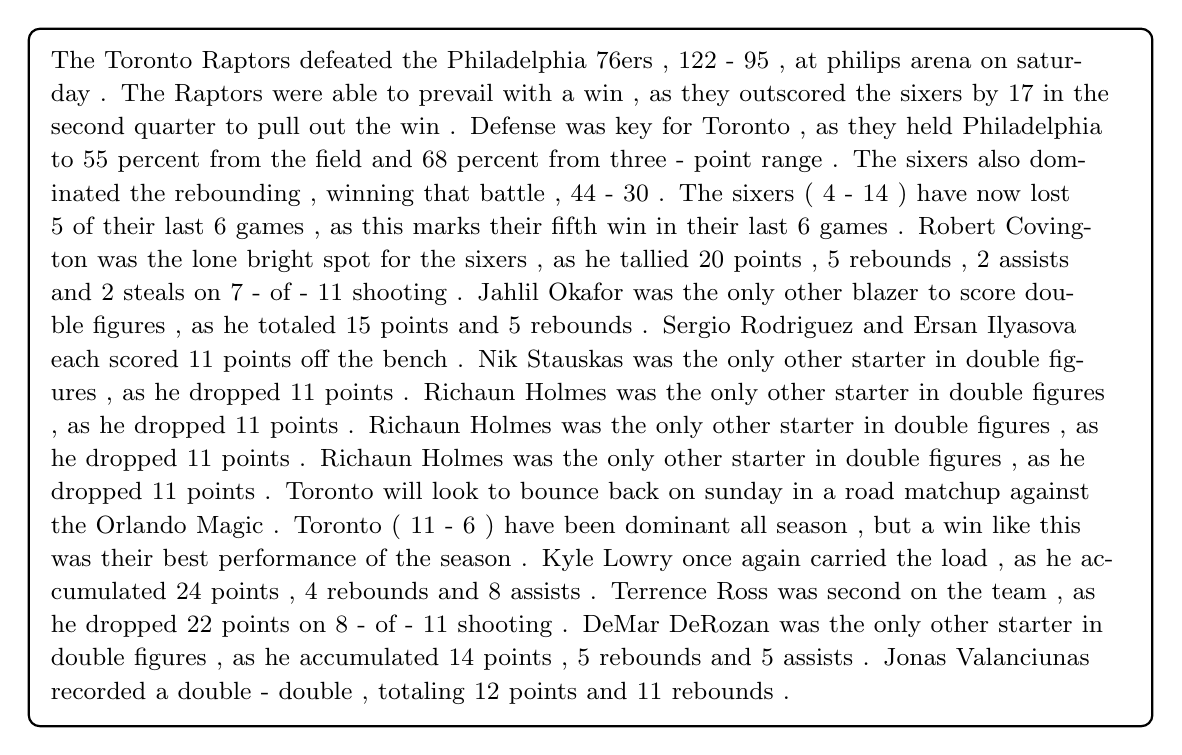
\begin{tikzpicture}
    \node(summary) [rectangle, draw,thick,fill=blue!0,text width=39em, rounded corners, inner sep =8pt, minimum height=1em]{
        \baselineskip=100pt
        \small
        The Toronto Raptors defeated the Philadelphia 76ers , 122 - 95 , at philips arena on saturday . The Raptors were able to prevail with a win , as they outscored the sixers by 17 in the second quarter to pull out the win . Defense was key for Toronto , as they held Philadelphia to 55 percent from the field and 68 percent from three - point range . The sixers also dominated the rebounding , winning that battle , 44 - 30 . The sixers ( 4 - 14 ) have now lost 5 of their last 6 games , as this marks their fifth win in their last 6 games . Robert Covington was the lone bright spot for the sixers , as he tallied 20 points , 5 rebounds , 2 assists and 2 steals on 7 - of - 11 shooting . Jahlil Okafor was the only other blazer to score double figures , as he totaled 15 points and 5 rebounds . Sergio Rodriguez and Ersan Ilyasova each scored 11 points off the bench . Nik Stauskas was the only other starter in double figures , as he dropped 11 points . Richaun Holmes was the only other starter in double figures , as he dropped 11 points . Richaun Holmes was the only other starter in double figures , as he dropped 11 points . Richaun Holmes was the only other starter in double figures , as he dropped 11 points . Toronto will look to bounce back on sunday in a road matchup against the Orlando Magic . Toronto ( 11 - 6 ) have been dominant all season , but a win like this was their best performance of the season . Kyle Lowry once again carried the load , as he accumulated 24 points , 4 rebounds and 8 assists . Terrence Ross was second on the team , as he dropped 22 points on 8 - of - 11 shooting . DeMar DeRozan was the only other starter in double figures , as he accumulated 14 points , 5 rebounds and 5 assists . Jonas Valanciunas recorded a double - double , totaling 12 points and 11 rebounds .
    };
    \end{tikzpicture} }
    \caption{\centering A summary generated by the Content Selection and Planning model from the gold content plans. The corresponding gold summary and input table is shown in figure \ref{figure:samplesummary}.} \label{figure:gold_cp_generated}
\end{figure}

The other generation setting is to use the generated content plans. However this is where we failed to obtain the same results as \citep{puduppully2019datatotext}. We observed that the network fails to learn when to place \emph{\textless EOS\textgreater} token in the content plan and the generated content plans end with sequence of repetitions. Therefore the part of the model responsible for text generation (Content Plan Encoder and Text Decoder) fails to generate reasonable texts. (Reasonable in terms of the used language. Table \ref{table:metrics_csap} shows that model still achieved reasonable entity recall (in fact better than any previous model) and the best correctness, although the correctness is due to large number of repetitions of the accurate information.)

\begin{table}[h]
    \centering
    \scalebox{0.8}{
    \begin{tabular}{lccccc}
        \toprule
        {} & \textbf{Validation} & \textbf{Validation} & \textbf{Test} & \textbf{Entity} & \textbf{Correct} \\
        \pulrad{\textbf{Model}} & \textbf{Perplexity$_1$} & \textbf{BLEU} & \textbf{BLEU} & \textbf{Recall} & \textbf{Facts} \\
        \midrule
        CS\&P$_G$ & {} & 13.07 & 13.08 & 44.58\% & 67.76\% \\
        CS\&P$_{G}^{*}$ & \pulrad{8.76} & 22.8$^{*}$ & -- & 71.43\%$^{*}$ & 54.69\%$^{*}$ \\
        \bottomrule
        \multicolumn{6}{l}{\footnotesize{CS\&P - Content Selection and Planning model}} \\
        \multicolumn{6}{l}{\footnotesize{$_{G}$ - Greedy Decoding}} \\
        \multicolumn{6}{l}{\footnotesize{$_1$ - Validation Perplexity of text decoded from gold content plans}} \\
        \multicolumn{6}{l}{\footnotesize{$^{*}$ - All the metrics are computed only on the validation part of the dataset, with \emph{gold content plans}}}
    \end{tabular}
    }
    \caption{Performance metrics on the Content Selection and Planning model.} \label{table:metrics_csap}
\end{table}
Since we do not implement the Beam Search decoder for the content plans (due to shortness of time) we try to artificially add \emph{\textless EOS\textgreater} token at some position in the generated content plan and mask everything after, however the results do not show any improvement. The same applies for using Beam Search in Text Decoder. 


\section{Ordered Tables}

Since we haven't managed to obtain sufficient results using any of the previously proposed methods we try to make the task easier. Looking at the results of the CS\&P model generating from the \emph{gold content plans}, we may draw a conclusion that the performance bottleneck is in the understanding of the tabular structure. Therefore in following sections we organize and reduce the size of the input tables, and observe the effects of these operations.

Going through the gold content plans as well as the ones generated by Content Selection and Planning model we spotted that their structure follows a simple pattern. At first the teams are presented, then there is some information about the best players and about players who performed surprisingly well.

Therefore we order the input records in a similar way. The first records in the ordered sequence belong to home and away teams. The remaining records contain information about all the players, who are ordered by their point-totals in the respective match.

\subsection{Results}

We trained only the Joint-Copy model on the ordered tables, and we cannot make any clear conclusions. We see a raise in terms of the BLEU score (of about $2$ points compared to Joint-Copy model trained on the original tables) but also a drop in both manually evaluated metrics. The overal performance of the model is comparable to Joint-Copy model with Content Selection Encoder. \emph{THE TRAINING OF THE CONTENT SELECTION MODEL IS STILL RUNNING, MAYBE THE CONCLUSIONS MAY CHANGE}.

\begin{table}[h]
    \centering
    \scalebox{0.8}{
    \begin{tabular}{lccccc}
        \toprule
        {} & \textbf{Validation} & \textbf{Validation} & \textbf{Test} & \textbf{Entity} & \textbf{Correct} \\
        \pulrad{\textbf{Model}} & \textbf{Perplexity} & \textbf{BLEU} & \textbf{BLEU} & \textbf{Recall} & \textbf{Facts} \\
        \midrule
        Copy$_{orderedG}$ & {} & 12.98 & 13.32 & -- & -- \\
        Copy$_{orderedB5}$ & \pulrad{9.21} & 13.75 & 14.01 & 33.73\% & 46.84\% \\
        \bottomrule
        \multicolumn{6}{l}{\footnotesize{Copy$_ordered$ - Joint-Copy model operating on the ordered tables}} \\
        \multicolumn{6}{l}{\footnotesize{$_{G}$ - Greedy Decoding}} \\
        \multicolumn{6}{l}{\footnotesize{$_{B5}$ - Beam search decoding, beam size $ = 5 $}} \\
    \end{tabular}
    }
    \caption{Performance metrics on the Content Selection and Planning model.} \label{table:metrics_copy_ordered}
\end{table}

\section{Shortened Tables} \label{section:shortened_tables}

We took the second effort to make the input tables easier to understand for the network. We order the tables as in previous section. Next we keep all the information about both teams and top three players according to their point totals. The information about the other players is reduced to minutes they played, points and assists they scored, their team and their name. The length of the new sequence of input records is $130$.

We opted to use an architecture similar to the one which achieved the best performance on the gold content plans. Following the notation from figure \ref{figure:overal_architecture_csap} we encode the records with Content Selection Encoder, next we use the Content Plan Encoder (bidirectional LSTM operating on the shortened sequences of records) and we feed its outputs to Text Decoder (which uses Joint-Copy mechanism). We call this model \emph{Copy$_{prunned}$}, its overall hyperparameter configuration is shown in figure \ref{figure:hyperparameters_copy_prunned}.

\begin{figure}[h]
    \scalebox{0.8}{
    \begin{tikzpicture}
    \node(embeddings) [] {
        \small
        \begin{tabular}{ll}
            \toprule
            {} & \textbf{Embedding} \\
            \pulrad{\textbf{Token}} & \textbf{Dimensionality} \\
            \midrule
            \textbf{$record.type$} & 300 \\
            \textbf{$record.home\_away$} & 300 \\
            \textbf{$record.value$} & 500 \\
            \textbf{$record.entity$} & 500 \\
            \textbf{$summary\ token$} & 500
        \end{tabular}
    };
    \node(hidden) [above left=-20.7mm and 5mm of embeddings] {
        \small
        \begin{tabular}{ccc}
            \toprule
            \textbf{Hidden States} & {} & {} \\
            \textbf{Dimensionality} & \pulrad{\textbf{Learning Rate}} & \pulrad{\textbf{Batch Size}} \\
            \midrule
            500 & 0.0002 & 8
        \end{tabular}
    };
    \end{tikzpicture}
    }
    \caption{Hyperparameter settings for Copy$_{prunned}$ models.} \label{figure:hyperparameters_copy_prunned}
\end{figure}

\subsection{Results}

This configuration (more sophisticated model, input table that is easier to understand) achieved the best BLEU score of all the models (excluding the one generating from the gold content plans). Table \ref{table:metrics_prunned} shows that we managed to improve the BLEU score by more than $1$ point compared to both CopyCS and Copy$_{ordered}$ models. Model also learned to mention more players, however not with correct statistics. Since we reduced the amount of input records related to all but the best three players, the model learned to \emph{hallucinate} the statements about the remainng ones. We haven't experimented with other possible combinations but we expect that the model performance would improve when about five best players would be fully described in the input tables (compared to actual three).

\begin{table}[h]
    \centering
    \scalebox{0.8}{
    \begin{tabular}{lccccc}
        \toprule
        {} & \textbf{Validation} & \textbf{Validation} & \textbf{Test} & \textbf{Entity} & \textbf{Correct} \\
        \pulrad{\textbf{Model}} & \textbf{Perplexity} & \textbf{BLEU} & \textbf{BLEU} & \textbf{Recall} & \textbf{Facts} \\
        \midrule
        Copy$_{prunnedG}$ & {} & 14.31 & 14.45 & -- & -- \\
        Copy$_{prunnedB5}$ & \pulrad{11.24} & 15.18 & 15.63 & 50.6\% & 49.87\% \\
        \bottomrule
        \multicolumn{6}{l}{\footnotesize{Copy$_prunned$ - the model introduced in section \ref{section:shortened_tables}}} \\
        \multicolumn{6}{l}{\footnotesize{$_{G}$ - Greedy Decoding}} \\
        \multicolumn{6}{l}{\footnotesize{$_{B5}$ - Beam search decoding, beam size $ = 5 $}} \\
    \end{tabular}
    }
    \caption{Performance metrics on the Content Selection and Planning model.} \label{table:metrics_prunned}
\end{table}

This is our final experiment, using the most advanced preprocessing as well as the most advanced model architecture. Therefore I would like to show how far is our best model from the ideal generation system described in the introduction. The generated text in figure \ref{figure:copy_prunned_generated} starts by introducing the teams that have played as well as the score and the location where the match was played. Next it contains some "interesting" events that happened, followed by statistics of the players. Many generated summaries (although not this one) end with a phrase about future schedule of both teams. Since \emph{Jahlil Okafor} isn't between the best three players of the match, \emph{all his statistics excluding his points and assists are hallucinated}. Model mixed up \emph{Robert Covington} with \emph{Terrence Ross}, thus the presented statistics are not correct. Overall we put our expectations too high and we are not able to come even close to any result that could have practical applications. 

\begin{figure}[h]
    \scalebox{0.85}{
    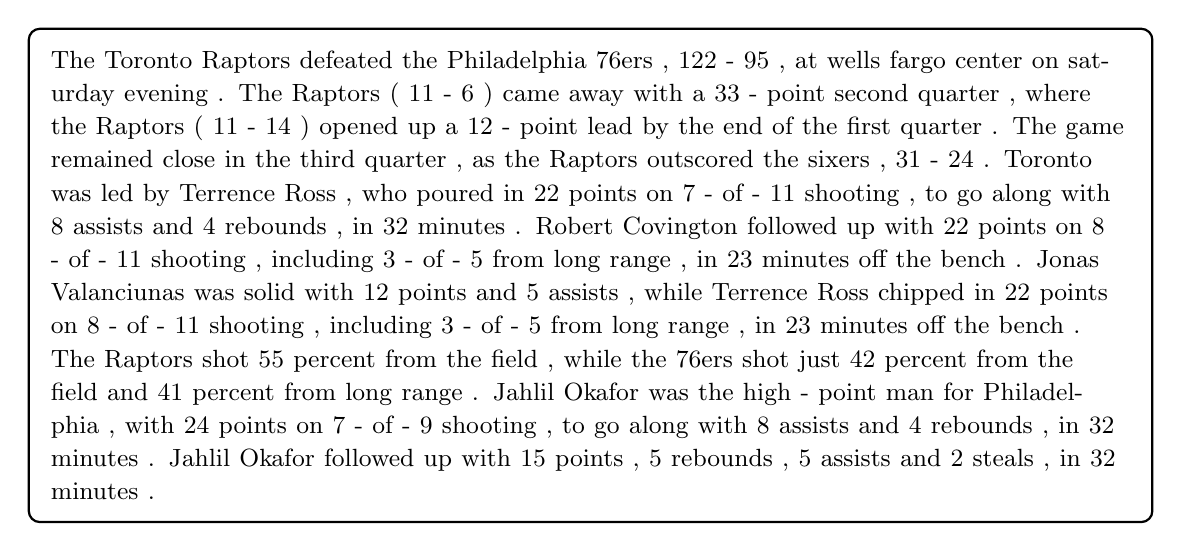
\begin{tikzpicture}
    \node(summary) [rectangle, draw,thick,fill=blue!0,text width=39em, rounded corners, inner sep =8pt, minimum height=1em]{
        \baselineskip=100pt
        \small
        The Toronto Raptors defeated the Philadelphia 76ers , 122 - 95 , at wells fargo center on saturday evening . The Raptors ( 11 - 6 ) came away with a 33 - point second quarter , where the Raptors ( 11 - 14 ) opened up a 12 - point lead by the end of the first quarter . The game remained close in the third quarter , as the Raptors outscored the sixers , 31 - 24 . Toronto was led by Terrence Ross , who poured in 22 points on 7 - of - 11 shooting , to go along with 8 assists and 4 rebounds , in 32 minutes . Robert Covington followed up with 22 points on 8 - of - 11 shooting , including 3 - of - 5 from long range , in 23 minutes off the bench . Jonas Valanciunas was solid with 12 points and 5 assists , while Terrence Ross chipped in 22 points on 8 - of - 11 shooting , including 3 - of - 5 from long range , in 23 minutes off the bench . The Raptors shot 55 percent from the field , while the 76ers shot just 42 percent from the field and 41 percent from long range . Jahlil Okafor was the high - point man for Philadelphia , with 24 points on 7 - of - 9 shooting , to go along with 8 assists and 4 rebounds , in 32 minutes . Jahlil Okafor followed up with 15 points , 5 rebounds , 5 assists and 2 steals , in 32 minutes .
    };
    \end{tikzpicture} }
    \caption{\centering A summary generated by the Copy$_{prunned}$ model. The corresponding gold summary and input table is shown in figure \ref{figure:samplesummary}.} \label{figure:copy_prunned_generated}
\end{figure}


\section{Overall Comparison}

We start with the Baseline model (section \ref{section:baseline_model}) which produces fairly good language but many hallucinated statements (only 8\% of the produced statements are correct).

Next we experiment with the Joint-Copy model (section \ref{section:copy_mechanism_intro}). There we see the number of correct statements to increase to more than 40\% and the BLEU score to rise by more than 2 points.

We move on to Joint-Copy model with Content Selection encoder ( section \ref{subsection:content_selection}). We see another improvement in the BLEU score (by 1 point) and the entity recall (by 5\%) however the number of correct facts decreases and the produced language contains many contradictions because we did not manage to find the right combination of the hyperparameters.

The Content Selection and Planning model (section \ref{section:content_selection_and_planning}) is the last one we use for the task. We see that the model achieves great performance on reduced and reorganized tables (the BLEU score bigger than 22) although the part of the model creating the reduced tables does not cooperate well with the part generating text, therefore we do not see any improvement over the Joint-Copy model with Content Selection encoder.

Our last experiments aim to make the sequence of input records more organized and shorter. We use a model introduced previously (Joint-Copy model) and another model with Content Selection encoder with bidirectional LSTM layer on the top and Joint-Copy decoder. On shortened and ordered tables we manage to increase the BLEU score by another point and all the manually evaluated metrics by at least 2 \%.

\begin{table}[h]
    \centering
    \scalebox{0.8}{
    \begin{tabular}{lccccc}
        \toprule
        {} & \textbf{Validation} & \textbf{Validation} & \textbf{Test} & \textbf{Entity} & \textbf{Correct} \\
        \pulrad{\textbf{Model}} & \textbf{Perplexity} & \textbf{BLEU} & \textbf{BLEU} & \textbf{Recall} & \textbf{Facts} \\
        \midrule
        BR$_{B5}$ & 10.59 & 9.99 & 10.6 & 37.35\% & 8.03\% \\
        Copy$_{B5}$ & 9.87 & 12.19 & 12.5 & 39.76\% & 47.13\% \\
        CopyCS$_{B5}$ & 9.93 & 13.54 & 13.96 & 44.58\% & 42.22\% \\
        CS\&P$_G$ & 8.76$^{*}$ & 13.07 & 13.08 & 44.58\% & 67.76\% \\
        Copy$_{orderedB5}$ & 9.21 & 13.75 & 14.01 & 33.73\% & 46.84\% \\
        Copy$_{prunnedB5}$ & 11.24 & 15.18 & 15.63 & 50.6\% & 49.87\% \\
        \bottomrule
        \multicolumn{6}{l}{\footnotesize{BR - Baseline, regularized}} \\
        \multicolumn{6}{l}{\footnotesize{Copy - Joint-Copy model}} \\
        \multicolumn{6}{l}{\footnotesize{CopyCS - Joint-Copy decoder $+$ Content Selection encoder}} \\
        \multicolumn{6}{l}{\footnotesize{CS\&P - Content Selection and Planning model}} \\
        \multicolumn{6}{l}{\footnotesize{Copy$_ordered$ - Joint-Copy model operating on the ordered tables}} \\
        \multicolumn{6}{l}{\footnotesize{Copy$_prunned$ - the model introduced in section \ref{section:shortened_tables}}} \\
        \multicolumn{6}{l}{\footnotesize{$_{G}$ - Greedy Decoding}} \\
        \multicolumn{6}{l}{\footnotesize{$_{B5}$ - Beam search decoding, beam size $ = 5 $}} \\
        \multicolumn{6}{l}{\footnotesize{$^{*}$ - Validation Perplexity of text decoded from gold content plans}} \\
    \end{tabular}
    }
    \caption{Performance metrics on all the models and approaches discussed in this chapter.} \label{table:metrics_all}
\end{table}

\section{Implementation Details}

As stated in the introduction this thesis is highly theoretical and experimental. The implementation serves as proof-of-concept and doesn't aim to be used in the production.

All the models and preprocessing methods were developed in \emph{python 3.8} and \emph{tensorflow 2.4.1}. However the code is compatible with \emph{python 3.6} and \emph{tensorflow 2.3} (the versions used on Artifical Intelligence Cluster (AIC) where the training was executed). The implementation is divided into two modules, \emph{preprocessing} and \emph{training}.

\subsection{Preprocessing Module}

The preprocessing happens in four steps.
\begin{enumerate}
    \item Filtering out the faulty data-points (section \ref{cleaning_section}) from the original dataset.
    \item Extraction and transformation of the summaries from the cleaned dataset.
    \item Byte Pair Encoding of the summaries. (As explained in section \ref{bpeSection} I use the \emph{subword-nmt} module by \citep{sennrich2016}.)
    \item Construction of the dataset from the encoded summaries and the cleaned data. 
\end{enumerate}
Each step is implemented in \emph{python} and the steps are connected by a shell script.

\subsection{Training Module}

The training module contains implementation of layers and models discussed in previous chapters as well as training, evaluation and inference methods. It makes use of \emph{graph execution}\footnote{\url{https://www.tensorflow.org/guide/intro_to_graphs}} during training and \emph{eager execution}\footnote{\url{https://www.tensorflow.org/guide/eager}} during evaluation and prediction.

The code is available at \url{https://github.com/gortibaldik/TTTGen/}.